\documentclass[final]{beamer}
%\usepackage[a1]{beamerposter}
\usetheme{umjiposter}
%\setlength{\paperwidth}{23.63in}
%\setlength{\paperheight}{35.44in}

%\setbeamercolor{block title}{fg=ngreen,bg=white} % Colors of the block titles
%\setbeamercolor{block body}{fg=black,bg=white} % Colors of the body of blocks
%\setbeamercolor{block alerted title}{fg=white,bg=dblue!70} % Colors of the highlighted block titles
%\setbeamercolor{block alerted body}{fg=black,bg=dblue!10} % Colors of the body of highlighted blocks

%\usepackage{booktabs} % Top and bottom rules for tables

%----------------------------------------------------------------------------------------
%	TITLE SECTION 
%----------------------------------------------------------------------------------------

\course{VE414 • Bayesian Analysis • Project}
\teamlogo{umjilogo.ong}
\title{Photoacoustic Ultrasound (PAUS) for \\[.1in] Co-Registered Imaging of Bone \\[.1in] Structure and Vasculature \\[.1in]} % Poster title
\author{Wang Xuanyu, Jiang Sifan, Wu Guangzheng} % Author(s)
\institute{Department and University Name} % Institution(s)
\instructor{Prof. Jing Liu}

%----------------------------------------------------------------------------------------

\begin{document}

\addtobeamertemplate{block end}{}{\vspace*{2ex}} % White space under blocks
\addtobeamertemplate{block alerted end}{}{\vspace*{2ex}} % White space under highlighted (alert) blocks

\setlength{\belowcaptionskip}{2ex} % White space under figures
\setlength\belowdisplayshortskip{2ex} % White space under equations

\begin{frame}

\begin{columns}[t]

\begin{column}{\marginwidth}\end{column} % Empty spacer column

\begin{column}{\colwidth} % The first column
\begin{tcolorbox}[width=\colwidth,height=\contentheight,top=.2in]
\begin{block}{Problem Statement}
Hidden trees are required to be estimated in a garden. Travellers can detect the number of fruits, which is produced by the hidden tree, near the traveller, at some certain position, and estimate the number of trees in the garden. 

\end{block}

\vspace{.5in}

\begin{block}{Data Visualization}
We use matplotlib to plot the data points from one trip in the figure. During each trip, the traveller only went through a certain part of the region, near the $y=x$ line. Regions showing the "nearest" result of different data points may also overlap with one another.

\vspace{.2in}

\begin{figure}[H]
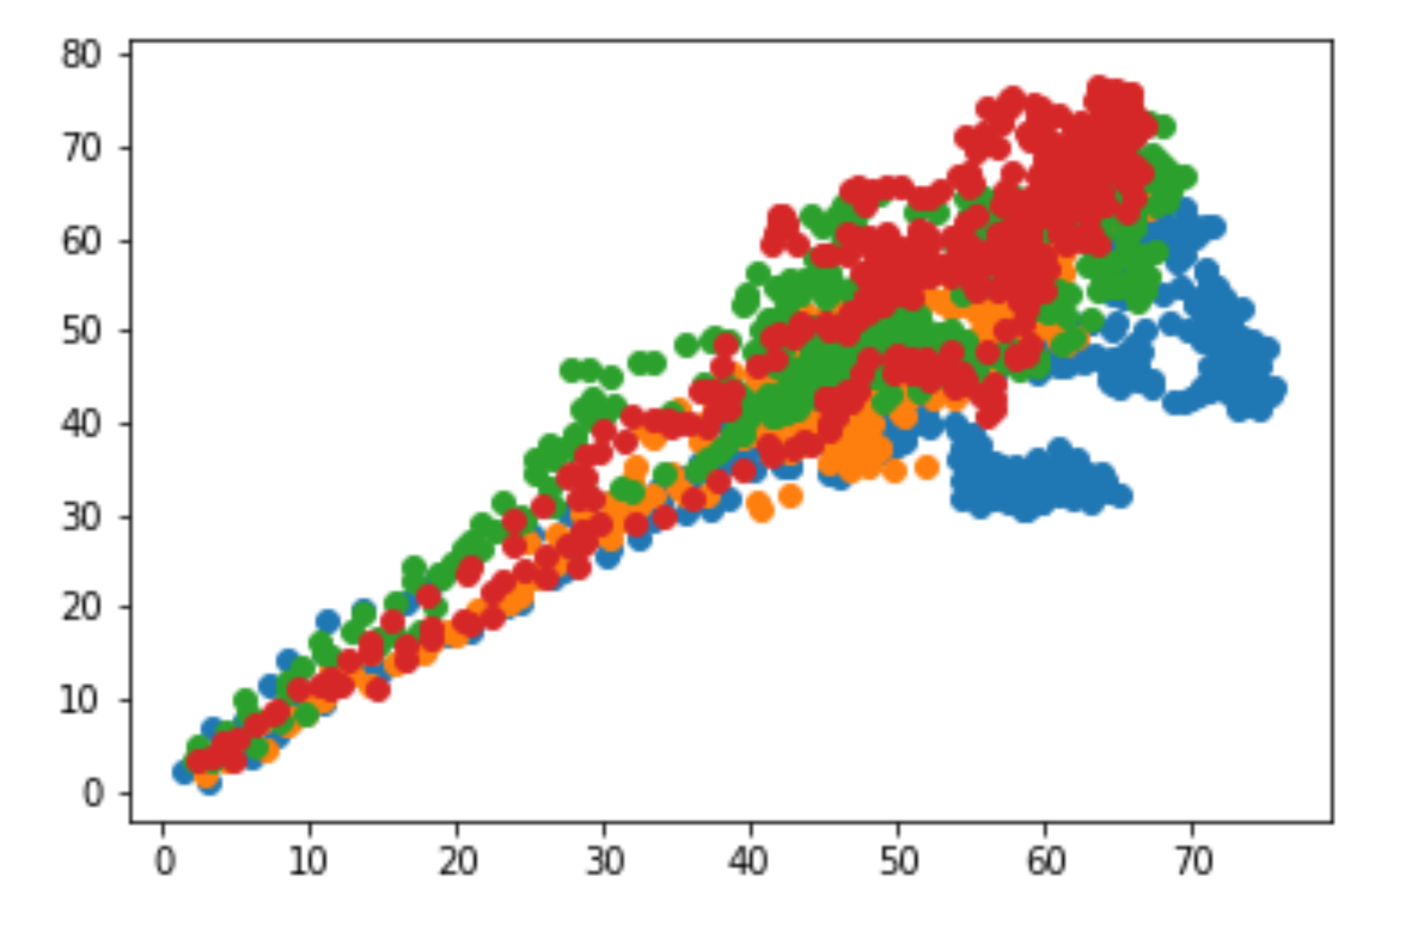
\includegraphics[width=1.0\textwidth]{data_points}
\caption{Plot of Data Points in Trip 1-4}
\end{figure}

Evidence can be provided to prove that the number and location of fruits didn't change in the whole process. That is, no extra fruit is produced by the hidden trees, and the travellers do not pick away the existing fruits.    

\end{block}

\vspace{.2in}

\begin{block}{Data Preprocessing}
Data Preprocessing is done in order to reduce the impact of errors and noise from the data. From the previous sections, we found that data points overlap with one another, making the fruits double-counted by different data points. Without data preprocessing, the estimated number of trees will be larger.

\end{block}

\end{tcolorbox}
\end{column}

\begin{column}{\marginwidth-\parsep}\end{column} % Empty spacer column

\begin{column}{\colwidth} % The second column
\begin{tcolorbox}[width=\colwidth,height=\contentheight,top=.2in]
\begin{block}{}


\begin{figure}[H]
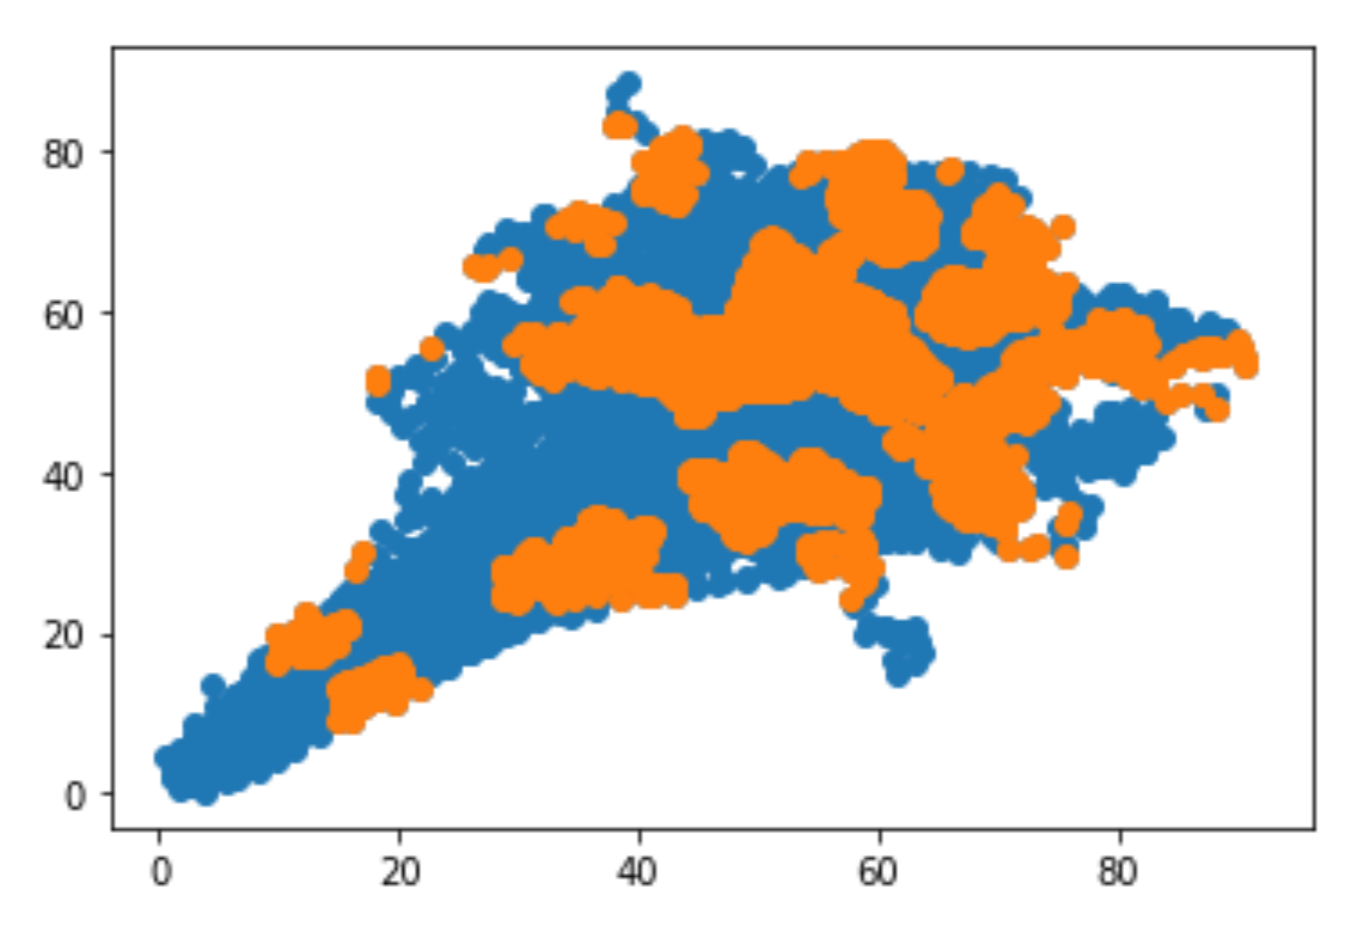
\includegraphics[width=1.0\textwidth]{data_points_overlap}
\caption{Data points overlap with each other}
\end{figure}

We reduced the number of data points by deleting some data points to avoid overlapping. Whenever two "close" regions overlap, the data points showing less fruit will be deleted, such that no space in the graden will be counted by two different data points.

\vspace{.2in}

\begin{figure}[H]
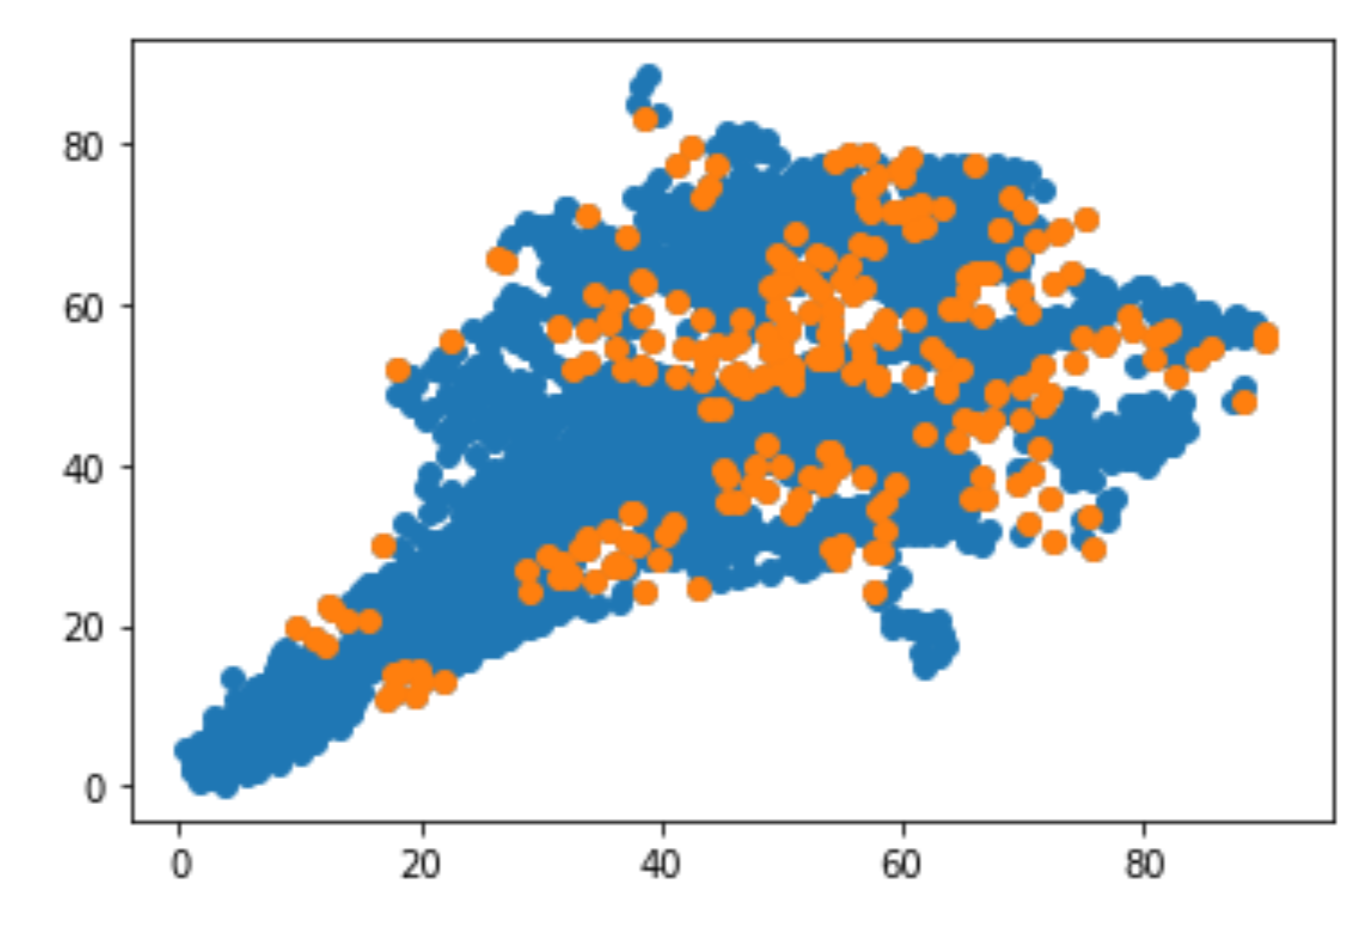
\includegraphics[width=0.9\textwidth]{data_points_cleaned}
\caption{Reduced Data Points without Overlap}
\end{figure}


\end{block}

\vspace{-.5in}

\begin{block}{Modeling and Analysis}
We use a Bayesian model to predict the number of trees. Suppose for every point in the whole garden, there is a probability density $p_k$ here that at this point a tree exist, such that the reject probability should be $1-p_k$ here.

\vspace{0.2in}

Since we had avoided the overlap, so we can imagine that for each data point, the place of the fruit follows a uniform distribution, and each fruit can be considered as a likelihood to update the posterior of $p_k$. A fruit will increase the probability of nearby $p_k$, while an empty data point will reject the probability $p_k$. 

\end{block}

\end{tcolorbox}
\end{column}

\begin{column}{\marginwidth-\parsep}\end{column} % Empty spacer column

\begin{column}{\colwidth} % The third column
\begin{tcolorbox}[width=\colwidth,height=\contentheight,top=.2in]
\begin{block}{}

\vspace{-.2in}

\begin{figure}[H]
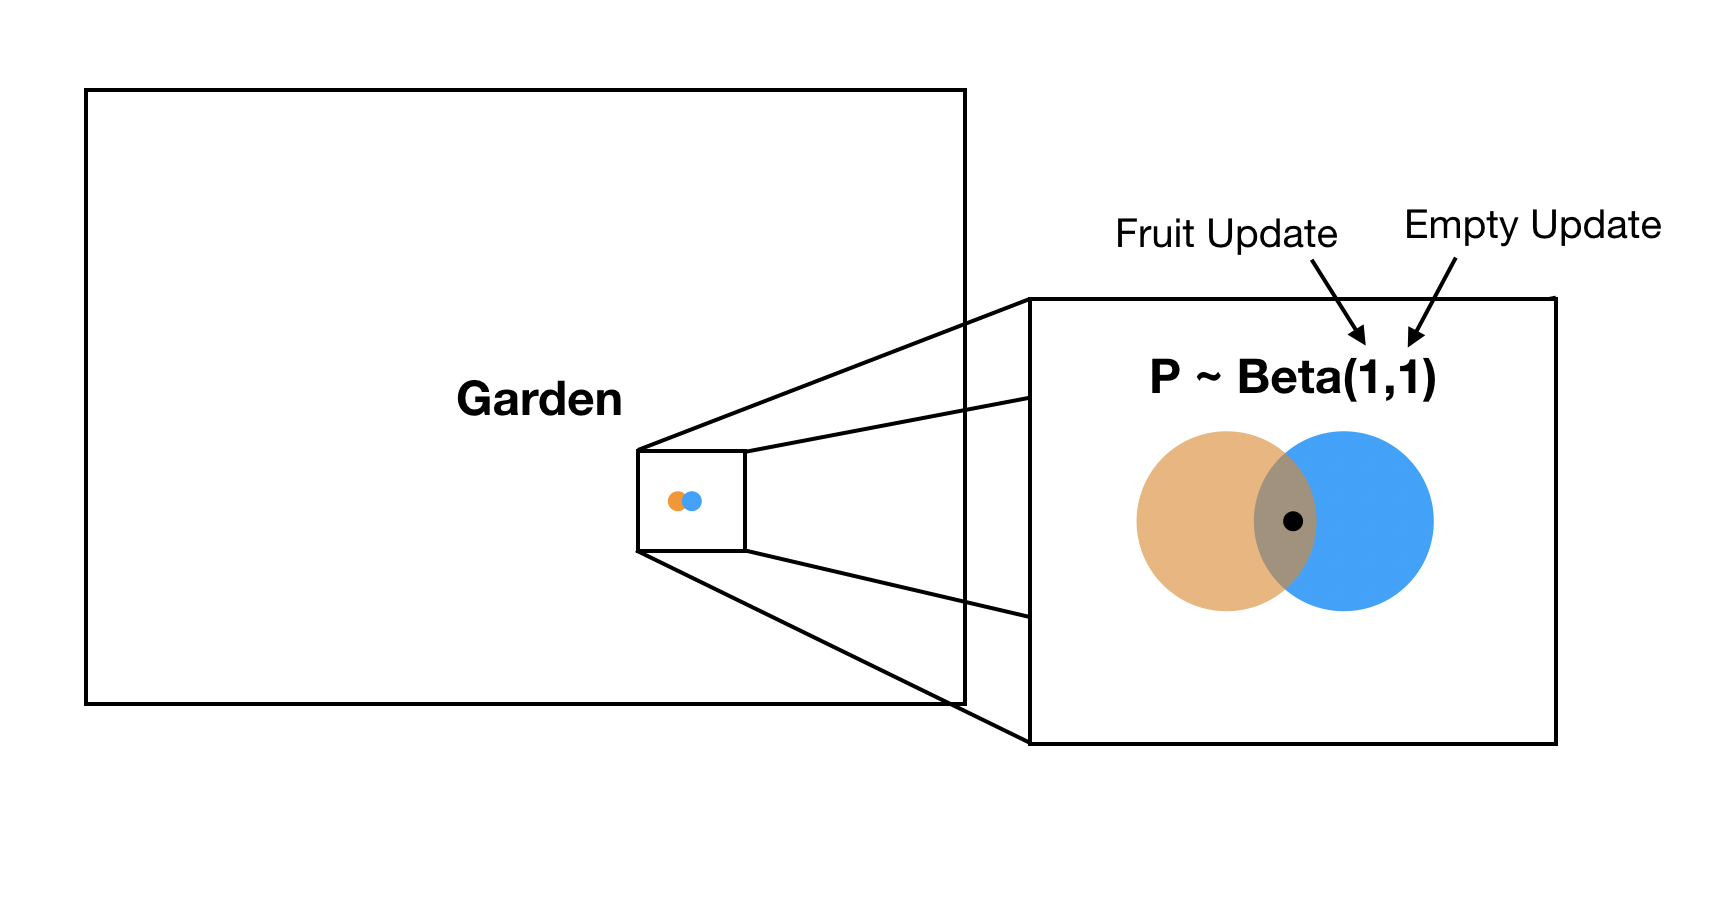
\includegraphics[width=0.9\textwidth]{model}
\caption{Our Bayesian Model}
\end{figure}

\vspace{-.3in}

The following table shows some parts of the resulted mean after an update of data points from the first trip. We can see that the points without being met remains unchanged, while probability density at point met the empty point was reduced.

\vspace{0.2in}
    
\begin{table}[H]
\centering
\begin{tabular}{|c|c|c|c|}
\hline
Point & 2 & 3 & 4\\
\hline
Position & $(0,2)$ & $(0,3)$ & $(0,4)$ \\
\hline 
Fruit & 0 & 0 & 0 \\
\hline
Empty & 0 & 0 & 1 \\
\hline
$\alpha$ & 1 & 1 & 1\\
\hline
$\beta$ & 1 & 1 & 2\\
\hline
mean & 0.500 & 0.500 & 0.333\\
\hline
\end{tabular}
\caption{$p_k$ after a First Update}
\end{table}

\vspace{-0.3in}

After the final update, we get a set of probability $p_k$ to as the sample of probability density. Each $p_k$ identifies the probability that at that point a tree is existed. The total number of trees should be the integral of the $p_k$ over the garden. We estimated that there are 169 trees that has been visited.

\vspace{0.1in}

The region visited is about $1/3$ to $1/2$ of the whole garden, which is shown in figure 2. So we estimated that there are about 400 trees in the garden.

\end{block}

\begin{block}{Conclusion}
This model provides a bayesian approach to predict the number of trees, which can also be applied to the situation where trees can move. Further improvement should be made to find a better way to deal with the overlap, since it is too strong and direct now.
\end{block}


\end{tcolorbox}
\end{column}

\begin{column}{\marginwidth}\end{column} % Empty spacer column

\end{columns}

\end{frame}


%\begin{frame}[t] % The whole poster is enclosed in one beamer frame
%
%\begin{columns}[t] % The whole poster consists of three major columns, the second of which is split into two columns twice - the [t] option aligns each column's content to the top
%
%\begin{column}{\sepwid}\end{column} % Empty spacer column
%
%\begin{column}{\onecolwid} % The first column
%
%%----------------------------------------------------------------------------------------
%%	OBJECTIVES
%%----------------------------------------------------------------------------------------
%
%\begin{alertblock}{Objectives}
%
%Lorem ipsum dolor sit amet, consectetur, nunc tellus pulvinar tortor, commodo eleifend risus arcu sed odio:
%\begin{itemize}
%\item Mollis dignissim, magna augue tincidunt dolor, interdum vestibulum urna
%\item Sed aliquet luctus lectus, eget aliquet leo ullamcorper consequat. Vivamus eros sem, iaculis ut euismod non, sollicitudin vel orci.
%\item Nascetur ridiculus mus.  
%\item Euismod non erat. Nam ultricies pellentesque nunc, ultrices volutpat nisl ultrices a.
%\end{itemize}
%
%\end{alertblock}
%
%%----------------------------------------------------------------------------------------
%%	INTRODUCTION
%%----------------------------------------------------------------------------------------
%
%\begin{block}{Introduction}
%
%Lorem ipsum dolor \textbf{sit amet}, consectetur adipiscing elit. Sed commodo molestie porta. Sed ultrices scelerisque sapien ac commodo. Donec ut volutpat elit. Sed laoreet accumsan mattis. Integer sapien tellus, auctor ac blandit eget, sollicitudin vitae lorem. Praesent dictum tempor pulvinar. Suspendisse potenti. Sed tincidunt varius ipsum, et porta nulla suscipit et. Etiam congue bibendum felis, ac dictum augue cursus a. \textbf{Donec} magna eros, iaculis sit amet placerat quis, laoreet id est. In ut orci purus, interdum ornare nibh. Pellentesque pulvinar, nibh ac malesuada accumsan, urna nunc convallis tortor, ac vehicula nulla tellus eget nulla. Nullam lectus tortor, \textit{consequat tempor hendrerit} quis, vestibulum in diam. Maecenas sed diam augue.
%
%Lorem ipsum dolor \textbf{sit amet}, consectetur adipiscing elit. Sed commodo molestie porta. Sed ultrices scelerisque sapien ac commodo. Donec ut volutpat elit. Sed laoreet accumsan mattis. Integer sapien tellus, auctor ac blandit eget, sollicitudin vitae lorem. Praesent dictum tempor pulvinar. Suspendisse potenti. Sed tincidunt varius ipsum, et porta nulla suscipit et. Etiam congue bibendum felis, ac dictum augue cursus a.
%
%This statement requires citation \cite{Smith:2012qr}.
%
%\end{block}
%
%%------------------------------------------------
%
%\begin{figure}
%\includegraphics[width=0.8\linewidth]{placeholder.jpg}
%\caption{Figure caption}
%\end{figure}
%
%%----------------------------------------------------------------------------------------
%
%\end{column} % End of the first column
%
%\begin{column}{\sepwid}\end{column} % Empty spacer column
%
%\begin{column}{\twocolwid} % Begin a column which is two columns wide (column 2)
%
%\begin{columns}[t,totalwidth=\twocolwid] % Split up the two columns wide column
%
%\begin{column}{\onecolwid}\vspace{-.6in} % The first column within column 2 (column 2.1)
%
%%----------------------------------------------------------------------------------------
%%	MATERIALS
%%----------------------------------------------------------------------------------------
%
%\begin{block}{Materials}
%
%The following materials were required to complete the research:
%
%\begin{itemize}
%\item Curabitur pellentesque dignissim
%\item Eu facilisis est tempus quis
%\item Duis porta consequat lorem
%\item Eu facilisis est tempus quis
%\end{itemize}
%
%The materials were prepared according to the steps outlined below:
%
%\begin{enumerate}
%\item Curabitur pellentesque dignissim
%\item Eu facilisis est tempus quis
%\item Duis porta consequat lorem
%\item Curabitur pellentesque dignissim
%\end{enumerate}
%
%\end{block}
%
%%----------------------------------------------------------------------------------------
%
%\end{column} % End of column 2.1
%
%\begin{column}{\onecolwid}\vspace{-.6in} % The second column within column 2 (column 2.2)
%
%%----------------------------------------------------------------------------------------
%%	METHODS
%%----------------------------------------------------------------------------------------
%
%\begin{block}{Methods}
%
%Lorem ipsum dolor \textbf{sit amet}, consectetur adipiscing elit. Sed laoreet accumsan mattis. Integer sapien tellus, auctor ac blandit eget, sollicitudin vitae lorem. Praesent dictum tempor pulvinar. Suspendisse potenti. Sed tincidunt varius ipsum, et porta nulla suscipit et. Etiam congue bibendum felis, ac dictum augue cursus a. \textbf{Donec} magna eros, iaculis sit amet placerat quis, laoreet id est. In ut orci purus, interdum ornare nibh. Pellentesque pulvinar, nibh ac malesuada accumsan, urna nunc convallis tortor, ac vehicula nulla tellus eget nulla. Nullam lectus tortor, \textit{consequat tempor hendrerit} quis, vestibulum in diam. Maecenas sed diam augue.
%
%\end{block}
%
%%----------------------------------------------------------------------------------------
%
%\end{column} % End of column 2.2
%
%\end{columns} % End of the split of column 2 - any content after this will now take up 2 columns width
%
%%----------------------------------------------------------------------------------------
%%	IMPORTANT RESULT
%%----------------------------------------------------------------------------------------
%
%\begin{alertblock}{Important Result}
%
%Lorem ipsum dolor \textbf{sit amet}, consectetur adipiscing elit. Sed commodo molestie porta. Sed ultrices scelerisque sapien ac commodo. Donec ut volutpat elit.
%
%\end{alertblock} 
%
%%----------------------------------------------------------------------------------------
%
%\begin{columns}[t,totalwidth=\twocolwid] % Split up the two columns wide column again
%
%\begin{column}{\onecolwid} % The first column within column 2 (column 2.1)
%
%%----------------------------------------------------------------------------------------
%%	MATHEMATICAL SECTION
%%----------------------------------------------------------------------------------------
%
%\begin{block}{Mathematical Section}
%
%Nam quis odio enim, in molestie libero. Vivamus cursus mi at nulla elementum sollicitudin. Nam quis odio enim, in molestie libero. Vivamus cursus mi at nulla elementum sollicitudin.
%  
%\begin{equation}
%E = mc^{2}
%\label{eqn:Einstein}
%\end{equation}
%
%Nam quis odio enim, in molestie libero. Vivamus cursus mi at nulla elementum sollicitudin. Nam quis odio enim, in molestie libero. Vivamus cursus mi at nulla elementum sollicitudin.
%
%\begin{equation}
%\cos^3 \theta =\frac{1}{4}\cos\theta+\frac{3}{4}\cos 3\theta
%\label{eq:refname}
%\end{equation}
%
%Nam quis odio enim, in molestie libero. Vivamus cursus mi at nulla elementum sollicitudin. Nam quis odio enim, in molestie libero. Vivamus cursus mi at nulla elementum sollicitudin.
%
%\begin{equation}
%\kappa =\frac{\xi}{E_{\mathrm{max}}} %\mathbb{ZNR}
%\end{equation}
%
%Nam quis odio enim, in molestie libero. Vivamus cursus mi at nulla elementum sollicitudin. Nam quis odio enim, in molestie libero. Vivamus cursus mi at nulla elementum sollicitudin.
%
%\end{block}
%
%%----------------------------------------------------------------------------------------
%
%\end{column} % End of column 2.1
%
%\begin{column}{\onecolwid} % The second column within column 2 (column 2.2)
%
%%----------------------------------------------------------------------------------------
%%	RESULTS
%%----------------------------------------------------------------------------------------
%
%\begin{block}{Results}
%
%\begin{figure}
%\includegraphics[width=0.8\linewidth]{placeholder.jpg}
%\caption{Figure caption}
%\end{figure}
%
%Nunc tempus venenatis facilisis. Curabitur suscipit consequat eros non porttitor. Sed a massa dolor, id ornare enim:
%
%Nunc tempus venenatis facilisis. Curabitur suscipit consequat eros non porttitor. Sed a massa dolor, id ornare enim:
%
%Nunc tempus venenatis facilisis. Curabitur suscipit consequat eros non porttitor. Sed a massa dolor, id ornare enim:
%
%Nunc tempus venenatis facilisis. Curabitur suscipit consequat eros non porttitor. Sed a massa dolor, id ornare enim:
%
%\begin{table}
%\vspace{2ex}
%\begin{tabular}{l l l}
%\toprule
%\textbf{Treatments} & \textbf{Res. 1} & \textbf{Res. 2}\\
%\midrule
%Treatment 1 & 0.0003262 & 0.562 \\
%Treatment 2 & 0.0015681 & 0.910 \\
%Treatment 3 & 0.0009271 & 0.296 \\
%\bottomrule
%\end{tabular}
%\caption{Table caption}
%\end{table}
%
%\end{block}
%
%%----------------------------------------------------------------------------------------
%
%\end{column} % End of column 2.2
%
%\end{columns} % End of the split of column 2
%
%\end{column} % End of the second column
%
%\begin{column}{\sepwid}\end{column} % Empty spacer column
%
%\begin{column}{\onecolwid} % The third column
%
%%----------------------------------------------------------------------------------------
%%	CONCLUSION
%%----------------------------------------------------------------------------------------
%
%\begin{block}{Conclusion}
%
%Nunc tempus venenatis facilisis. \textbf{Curabitur suscipit} consequat eros non porttitor. Sed a massa dolor, id ornare enim. Fusce quis massa dictum tortor \textbf{tincidunt mattis}. Donec quam est, lobortis quis pretium at, laoreet scelerisque lacus. Nam quis odio enim, in molestie libero. Vivamus cursus mi at \textit{nulla elementum sollicitudin}.
%
%Nunc tempus venenatis facilisis. Curabitur suscipit consequat eros non porttitor. Sed a massa dolor, id ornare enim.
%
%\end{block}
%
%%----------------------------------------------------------------------------------------
%%	ADDITIONAL INFORMATION
%%----------------------------------------------------------------------------------------
%
%\begin{block}{Additional Information}
%
%Maecenas ultricies feugiat velit non mattis. Fusce tempus arcu id ligula varius dictum. 
%\begin{itemize}
%\item Curabitur pellentesque dignissim
%\item Eu facilisis est tempus quis
%\item Duis porta consequat lorem
%\end{itemize}
%
%Maecenas ultricies feugiat velit non mattis. Fusce tempus arcu id ligula varius dictum. 
%\begin{itemize}
%\item Curabitur pellentesque dignissim
%\item Eu facilisis est tempus quis
%\item Duis porta consequat lorem
%\end{itemize}
%
%\end{block}
%
%%----------------------------------------------------------------------------------------
%%	REFERENCES
%%----------------------------------------------------------------------------------------
%
%\begin{block}{References}
%
%\nocite{*} % Insert publications even if they are not cited in the poster
%\small{\bibliographystyle{unsrt}
%\bibliography{sample}\vspace{0.75in}}
%
%\end{block}
%
%%----------------------------------------------------------------------------------------
%%	ACKNOWLEDGEMENTS
%%----------------------------------------------------------------------------------------
%
%\setbeamercolor{block title}{fg=red,bg=white} % Change the block title color
%
%\begin{block}{Acknowledgements}
%
%\small{\rmfamily{Nam mollis tristique neque eu luctus. Suspendisse rutrum congue nisi sed convallis. Aenean id neque dolor. Pellentesque habitant morbi tristique senectus et netus et malesuada fames ac turpis egestas.}} \\
%
%\end{block}
%
%%----------------------------------------------------------------------------------------
%%	CONTACT INFORMATION
%%----------------------------------------------------------------------------------------
%
%\setbeamercolor{block alerted title}{fg=black,bg=norange} % Change the alert block title colors
%\setbeamercolor{block alerted body}{fg=black,bg=white} % Change the alert block body colors
%
%\begin{alertblock}{Contact Information}
%
%\begin{itemize}
%\item Web: \href{http://www.my.edu/smithlab}{http://www.my.edu/smithlab}
%\item Email: \href{mailto:john@smith.com}{john@smith.com}
%\item Phone: +1 (000) 111 1111
%\end{itemize}
%
%\end{alertblock}
%
%\begin{center}
%\begin{tabular}{ccc}
%\includegraphics[width=0.4\linewidth]{logo.png} & \hfill & \includegraphics[width=0.4\linewidth]{logo.png}
%\end{tabular}
%\end{center}
%
%%----------------------------------------------------------------------------------------
%
%\end{column} % End of the third column
%
%\end{columns} % End of all the columns in the poster
%
%\end{frame} % End of the enclosing frame
%
\end{document}
